\documentclass[border=10pt]{standalone}

\usepackage{tikz}
\usepackage{tikzsymbols}
\usetikzlibrary{calc,patterns,shapes.geometric}

\def\centerarc[#1](#2)(#3:#4:#5){\draw[#1] ($(#2)+({#5*cos(#3)},{#5*sin(#3)})$) arc (#3:#4:#5);}

\begin{document}
	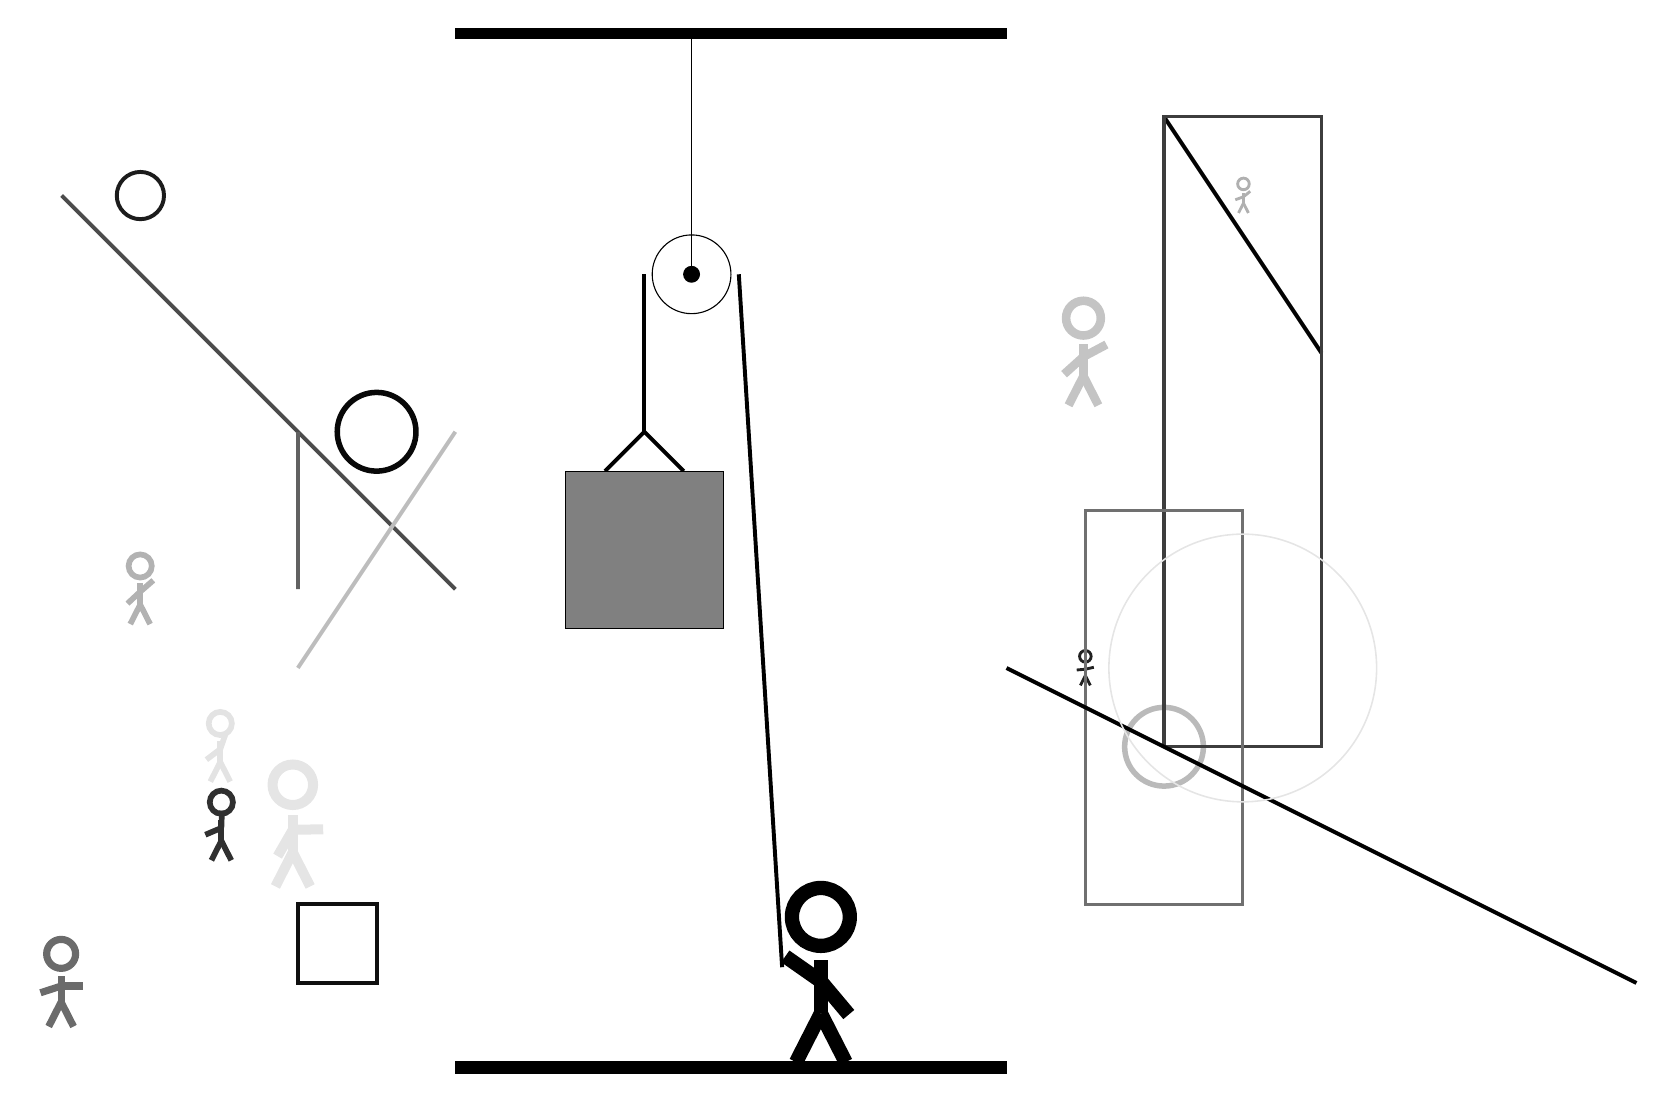
\begin{tikzpicture}
		%%%%% START %%%%%
		
		\draw[fill=black] (-2, 10) rectangle (5, 10.125);
		
		\draw (1, 7) circle (0.5);
		\draw[fill=black] (1, 7) circle (0.1);
		\draw (1, 10) -- (1, 7);
		
		\draw[line width=0.5mm] (-0.1, 4.5) -- (0.4, 5.0) -- (0.9, 4.5);
		\draw[fill=black!50] (-0.6, 4.5) rectangle (1.4, 2.5);
		
		\draw[line width=0.5mm] (0.4, 7) -- (0.4, 5.0);
		\centerarc[line width=0.5mm](1, 7)(0:180:0.6);
		\draw[line width=0.5mm](1.6, 7) -- (2.15, -1.8);
		
		\node[line width=0.5mm, color=black!87] at (6, 2) {\Strichmaxerl[2][5][13]};
		
		\draw [line width=0.7mm, color=black!27](7, 1) circle (0.5);
		\draw[line width=0.5mm, color=black!70](-7, 8) -- (-2, 3);
		\draw[line width=0.5mm, color=black!99](7, 9) -- (9, 6);
		
		\node[line width=0.5mm, color=black!58] at (-7, -2) {\Strichmaxerl[5][18][0]};
		\draw [line width=0.5mm, color=black!89](-6, 8) circle (0.3);
		\node[line width=0.5mm, color=black!10] at (-4, 0) {\Strichmaxerl[7][60][1]};
		
		\draw[line width=0.5mm, color=black!62] (-4, 3) rectangle (-4, 5);
		\draw[line width=0.4mm, color=black!76] (7, 9) rectangle (9, 1);
		\draw[line width=0.4mm, color=black!56] (6, 4) rectangle (8, -1);
		\draw[line width=0.5mm, color=black!100](5, 2) -- (13, -2);
		
		\draw [line width=0.2mm, color=black!10](8, 2) circle (1.7);
		\node[line width=0.5mm, color=black!23] at (6, 6) {\Strichmaxerl[6][42][28]};
		
		\draw[line width=0.5mm, color=black!26](-4, 2) -- (-2, 5);
		\node[line width=0.2mm, color=black!81] at (-5, 0) {\Strichmaxerl[4][23][88]};
		\draw [line width=0.7mm, color=black!97](-3, 5) circle (0.5);
		
		\node[line width=0.3mm, color=black!11] at (-5, 1) {\Strichmaxerl[4][37][71]};
		\draw[line width=0.5mm, color=black!94] (-3, -2) rectangle (-4, -1);
		\node[line width=0.2mm, color=black!30] at (-6, 3) {\Strichmaxerl[4][43][41]};
		\node[line width=0.3mm, color=black!31] at (8, 8) {\Strichmaxerl[2][20][39]};
		
		\node at (2.6, -1.9) {\Strichmaxerl[10][-35][-50]};
		
		\draw[fill=black] (-2, -3) rectangle (5, -3.15);
		
		%%%%% END %%%%%
	\end{tikzpicture}
\end{document}